\section{A simulated example from healthcare}
\label{sec:simulated_example}
Given the results in \cref{sec:real_example}, natural questions arise. For example, are such conclusion reversals specific to the explained component? Are these reversals always consequences of model misspecification or sampling variability? Here, we present a simulated example inspired by real-life healthcare data.
Our example exhibits sign reversals in the \emph{unexplained} component of the OBD under correct model specification and population-level parameters.

% To illustrate why \cref{eq:ob_decomp_ref_group} can lead a practitioner to draw substantially different conclusions depending on the reference group used in the OBD, we turn to a simple simulated healthcare example inspired by real-life data.

\textbf{Motivation.}
While our example is purely simulated, it is motivated by the following real-life concerns and observations.
Body mass index (BMI) is a widely recognized and routinely measured marker of wellness \cite{heymsfield2016} and is strongly linked to cardiometabolic outcomes, such as elevated blood pressure \cite{brown2000body}.
A researcher studying cardiac health may use commonly observed covariates like BMI to investigate whether differences in blood pressure between two groups are explainable by differences in basic markers of health between the groups, or differences in how these markers map to blood pressure.

Our example imagines two groups of adults in primary care being followed for elevated blood pressure, using systolic blood pressure (SBP) at a follow-up visit as the outcome $Y$. The BMI ($X$) of each adult is measured at an intake visit.
The first, Group $H$, comes from a higher-resource setting, such as an urban neighborhood with structured care pathways, frequent follow up, and better access to healthy food options. 
The second, Group $K$, comes from a lower-resource setting, where patients face barriers such as longer travel to clinics, infrequent follow up, and limited access to nutritious food.
These factors shape both the composition of each group (including average BMI) and the structure of the SBP--BMI relationship. We follow a clinical literature finding an approximately linear relationship between BMI and SBP \cite{kaufman1997, cappuccio2008, chen2023}; in particular, we assume a separate linear relationship in each group.

While an OBD cannot establish causality without further assumptions, it can suggest where one might look for potential drivers of observed inter-group disparities.
If the explained component is effectively zero and the unexplained component (differences in $Y \mid X$) dominates (with a sign in the direction of the observed outcome difference), it may highlight the need to investigate differences in medical care, such as adherence support or access to antihypertensives.
If the unexplained component is effectively zero and the explained component (differences in $X$) dominates (with a sign in the direction of the observed outcome difference), it may be most impactful to target interventions on weight management, nutrition, and physical activity. 

\textbf{Simulated data.}
We generate the BMI ($X$, in kg/m$^2$) of an individual in group \( g \) from a group-specific normal distribution.
We generate the SBP ($Y$, in mmHg) of an individual in group \( g \) as a noisy function of their BMI:
\begin{equation}
    \label{eq:linear_model}
   Y = \alpha_g + X \beta_g + \varepsilon.
\end{equation}
Here $\alpha_g \in \mathbb{R}$ is the group-specific intercept (in units of mmHg); $\beta_g \in \mathbb{R}$ is the group-specific slope, representing the average change in SBP (mmHg) per unit increase in BMI (kg/m$^2$); and $\varepsilon$ reflects individual variability in SBP that is uncorrelated with BMI. We take $\varepsilon$ independent and identically distributed across adult patients, with the same (mean-zero Gaussian) distribution in each group.
We present key parameters in \cref{tab:dgp_short} and provide further details about the data-generating process in \cref{appendix:dgp}.

\begin{table}[h]
\caption{Key chosen and derived parameters by group. BMI and SBP are in kg/m$^2$ and mmHg respectively. $\alpha$ is in mmHg; $\beta$ is in mmHg per kg/m$^2$.}
\label{tab:dgp_short}
\begin{center}
\small
\begin{tabular}{lcccc}
\toprule
Group & Mean BMI & $\alpha$ & $\beta$ & Mean SBP \\
\midrule
$H$ & 25.0 & 110.4 & 1.0 & 135.4 \\
$K$ & 27.0 & 100.0 & 1.4 & 137.8 \\
\bottomrule
\end{tabular}
\end{center}
\vskip -0.1in
\end{table}

\cref{fig:bmi_sbp} shows the population SBP--BMI relationships for both groups (two lines). The figure also shows data samples
to illustrate the BMI distribution in each group --- as well as how the intercepts, slopes, and BMI distributions interact.
%
Overall, Group $H$ has lower average SBP than Group $K$, owing both to lower average BMI and a shallower slope relating BMI to SBP, perhaps reflecting improved access and adherence to treatment, or availability of non-pharmacological support.
However, Group $H$ has a higher baseline SBP ($\alpha_H$), perhaps reflecting genetic factors in Group $H$.

\begin{figure}[h]
\centerline{
\includegraphics[width=0.5\linewidth]{Sections/Figures/bmi_sbp_comparison_population.pdf}}
\caption{Population linear models of SBP on BMI by group and data samples.}
\label{fig:bmi_sbp}
\end{figure}

\textbf{Analysis.} Since we have access to all population quantities in this example, there is no need to fit models or check statistical significance.
We can compute the OBD directly from the known population distributions.
%In principle, the OBD should provide a transparent framework to separate the difference in mean SBP into an explained component (differences in BMI distribution, $X$) and an unexplained component (differences in SBP given BMI, $Y \mid X$)

\textbf{Two different conclusions.}
\cref{tab:ob_decomp} summarizes the OBD results under each reference group.
For both choices of reference group the explained components are negative, so both choices of reference imply that $H$'s lower average SBP is due in part to its lower average BMI.
However, the sign of the unexplained OBD component flips depending on the choice of the reference group.
When group $H$ is the reference, the negative unexplained component implies that institutional factors further reduce group $H$'s blood pressure relative to group $K$.
However, when group $K$ is the reference, institutional factors appear to actually \emph{increase} group $H$'s average blood pressure relative to group $K$.
Intuitively, because blood pressure in group $K$ is so much more responsive to BMI, group $H$'s lower average BMI appears so good as to ``over-explain'' the difference in SBP; the unexplained component is then forced to be positive to compensate.

In this example, the sign change is in the unexplained component rather than the explained component (cf.\ \cref{sec:real_example}). Since we simulate the data according to group-specific linear models, there is no misspecification. And since we work directly with population quantities, the difference in OBD conclusions is not a product of sampling error.

\begin{table}[H]
\caption{Population Oaxaca–Blinder decomposition of mean SBP differences. All values are in mmHg.}
\label{tab:ob_decomp}
\begin{center}
\small
\begin{tabular}{lrrr}
\toprule
Reference & Explained & Unexplained & Total gap \\
\midrule
$H$ & $-2.0$ & $\textbf{-0.4}$ & $-2.4$ \\
$K$ & $-2.8$ & $\textbf{0.4}$  & $-2.4$ \\
\bottomrule
\end{tabular}
\end{center}
\vskip -0.1in
\end{table}

% \begin{table}[H]
% \caption{Estimated Oaxaca–Blinder decomposition of mean SBP differences}
% \label{tab:ob_decomp}
% \begin{center}
% \small
% \begin{tabular}{lrrr}
% \textbf{Group} & \textbf{Explained} & \textbf{Unexplained} & \textbf{Total gap} \\
% \hline \\
% H & $-1.91$ & $\textbf{-0.14}$ & $-2.05$ \\
% K & $-2.61$ & $\textbf{0.57}$  & $-2.05$ \\
% \end{tabular}
% \end{center}
% \footnotesize{Note: H = Higher-resource group, K = Lower-resource group. All values in mmHg.}
% \end{table}

%\begin{figure*}[t]
%\vspace{.3in}
%\centerline{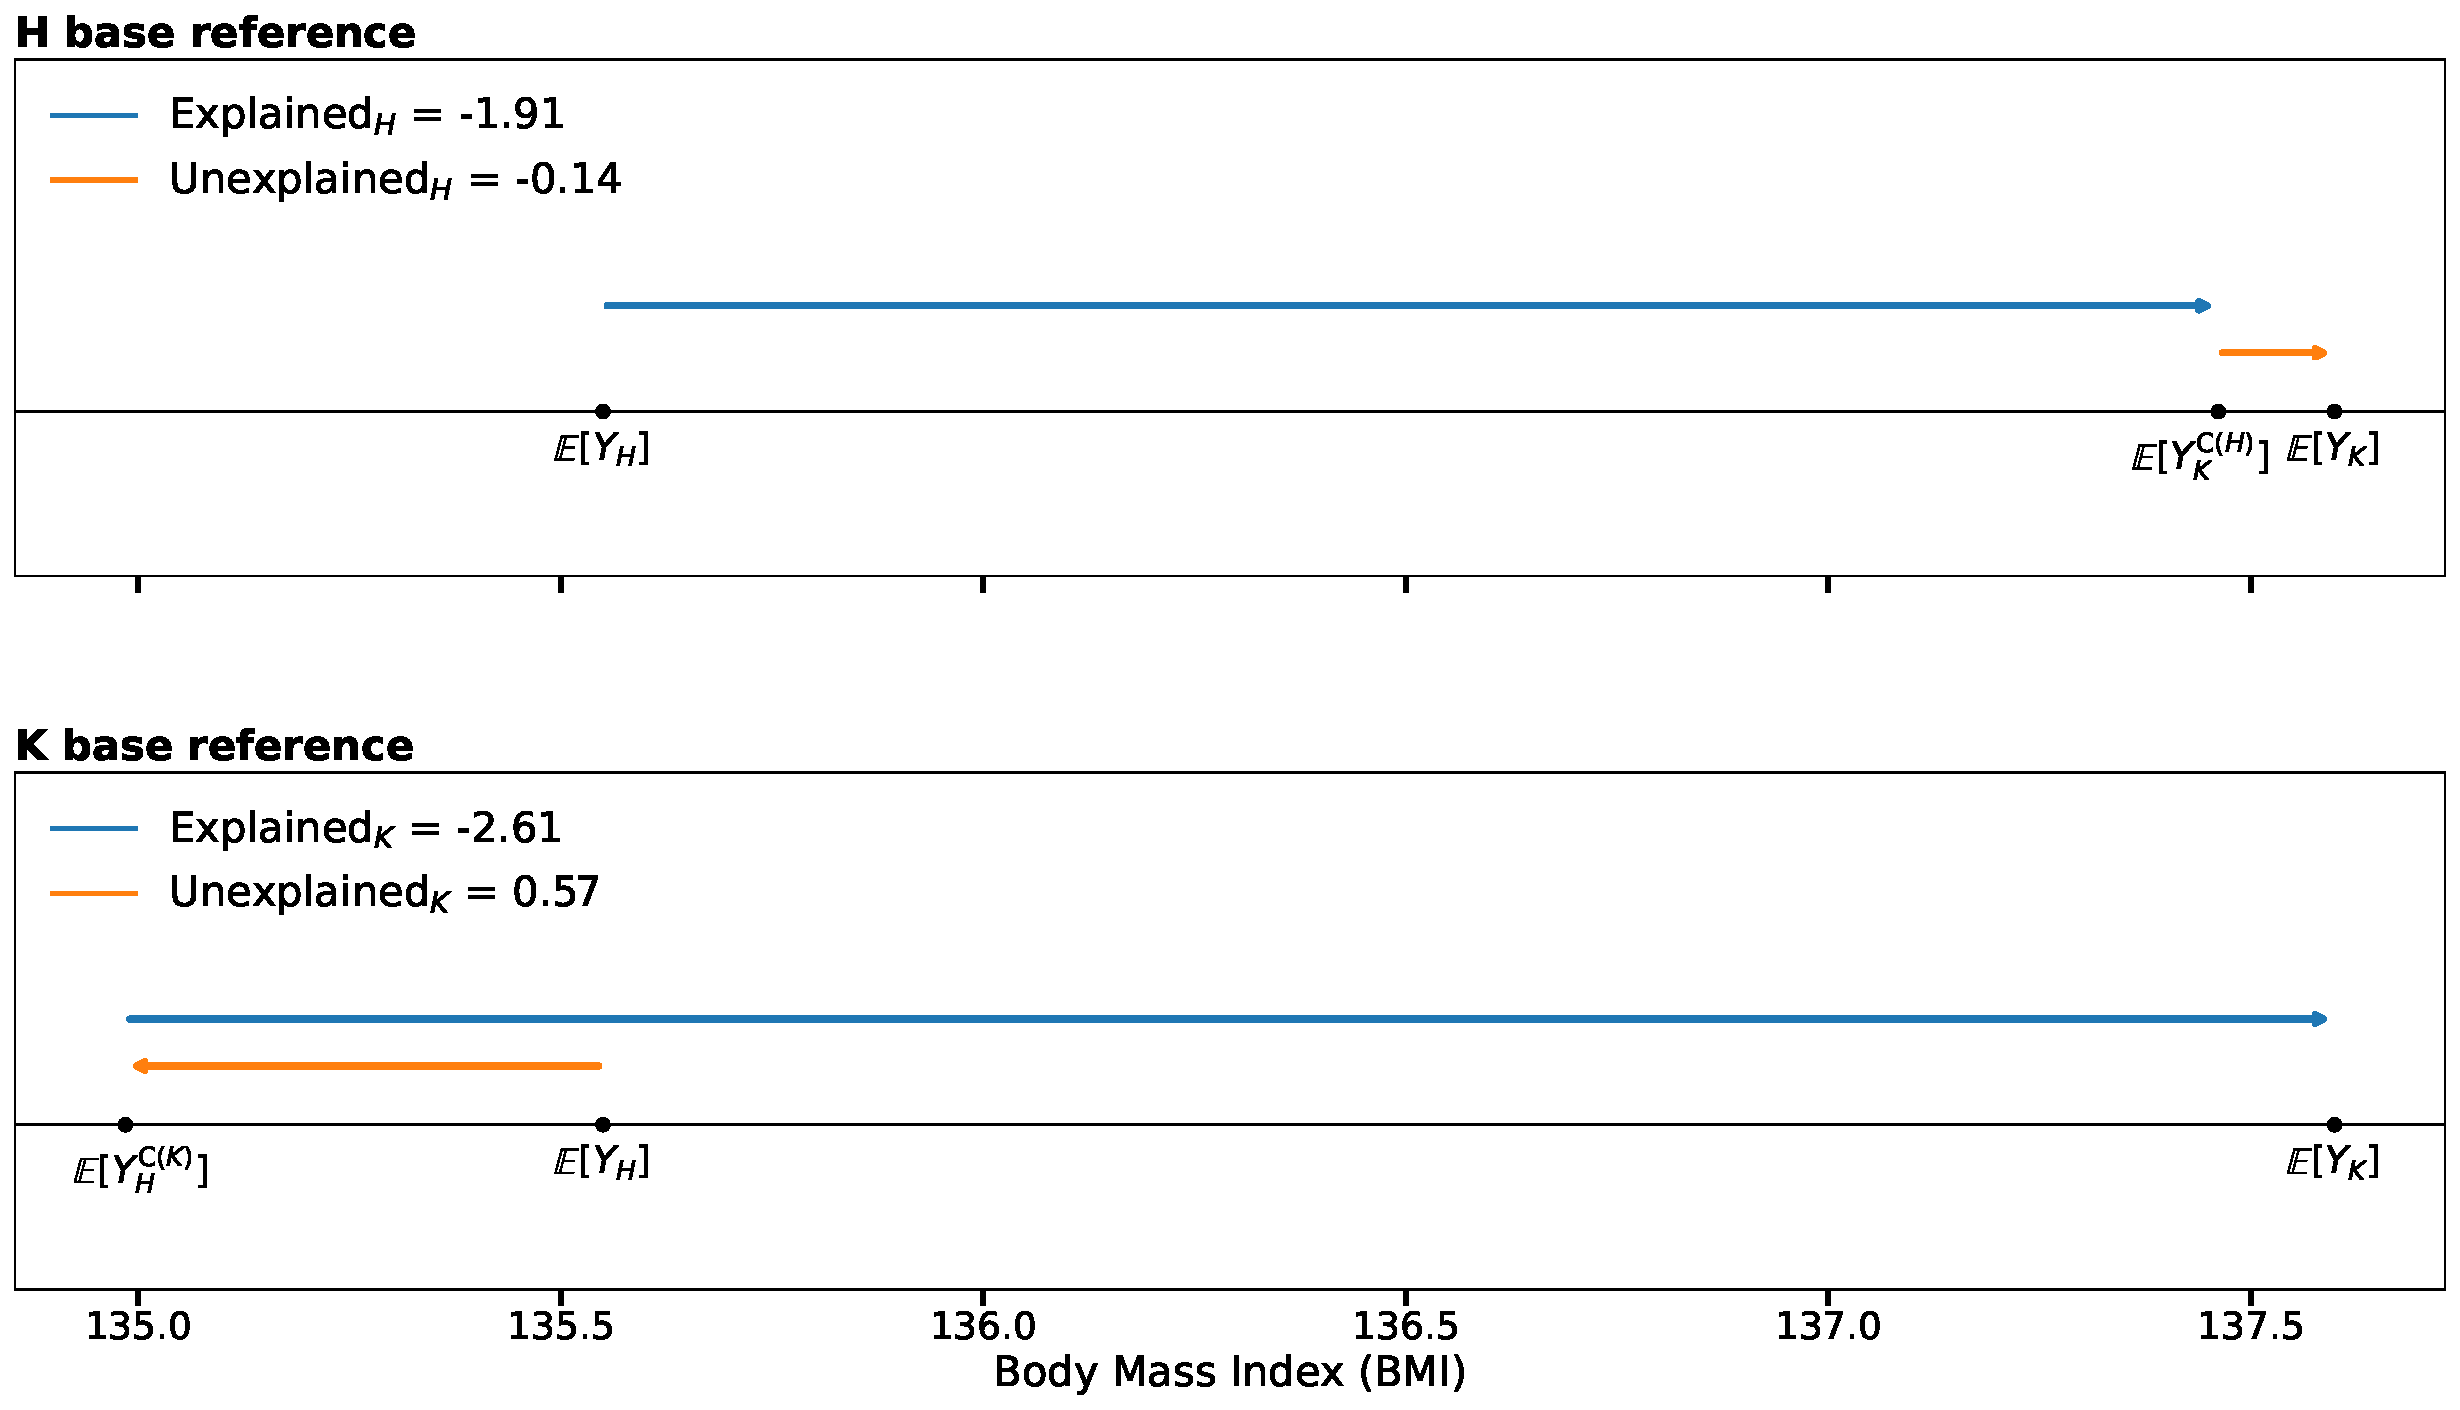
\includegraphics[width=0.7\textwidth]{Sections/Figures/counterfactual.pdf}}
%\vspace{.3in}
%\caption{Counterfactual analysis visualization showing the decomposition results for both reference groups in our simulated example.}
%\label{fig:counterfactual}
%\end{figure*}

%\cref{fig:counterfactual} visualizes the OBD as the mere difference between the counterfactual question posed by each choice of reference group and the observed mean SBP for each group. It also illustrates the sign flip in the unexplained component.

% \textcolor{red}{mega double check conclusion:}
% Some authors might argue that the choice of reference group simply reflects a different counterfactual question, for example, ``What would the SBP gap be if the lower resource group had the BMI--SBP relationship of the higher resource group?'' versus ``What would the gap be if the higher resource group had the BMI--SBP relationship of the lower resource group?'' 
% Others might claim that the true effect lies somewhere between these two extremes, and that averaging across reference groups provides a balanced view. 
% However, in our setting we argue that such sensitivity is problematic: when the sign of the unexplained component reverses, the qualitative policy message changes, creating a real risk of misinterpretation rather than a benign difference in framing.


